\section{Modelli utilizzati}
\subsection{RNN}
Una rete neurale ricorrente \`e una rete in cui esistono cammini trai nodi che formano dei cicli. Il tipo utilizzato in questa tesi \`e Long Short Term Memory (LSTM). Una rete LSTM, composta da neuroni LSTM, ha la capacit\`a di ricordare gli elementi passati per un determinato tempo, quindi per un certo numero di attivazioni, ed \`e quindi indicata in problemi dove ci sono da imparare sequenze e visto che nel problema affrontato devono essere imparate sequenze di note \`e sembrata la pi\`u appropriata. Il grafo che la rappresenta \`e il seguente:
\tikzset{%
  every neuron/.style={
    circle,
    draw,
    minimum size=1cm
  },
  neuron missing/.style={
    draw=none, 
    scale=4,
    text height=0.333cm,
    execute at begin node=\color{black}$\vdots$
  },
}
\begin{center}
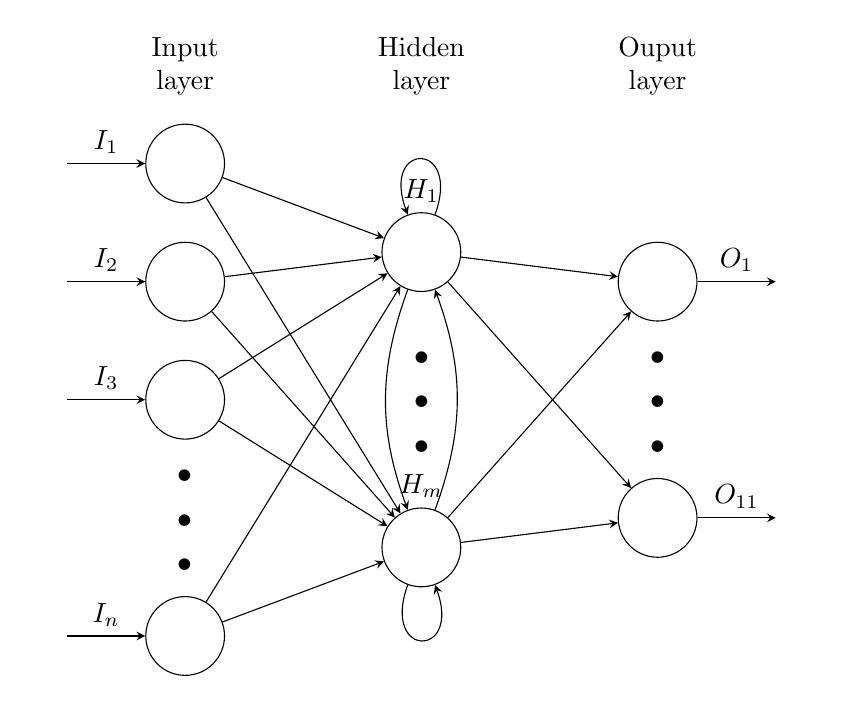
\begin{tikzpicture}[x=1.5cm, y=1.5cm, >=stealth]

\foreach \m/\l [count=\y] in {1,2,3,missing,4}
  \node [every neuron/.try, neuron \m/.try] (input-\m) at (0,2.5-\y) {};

\foreach \m [count=\y] in {1,missing,2}
  \node [every neuron/.try, neuron \m/.try ] (hidden-\m) at (2,2-\y*1.25) {};

\foreach \m [count=\y] in {1,missing,2}
  \node [every neuron/.try, neuron \m/.try ] (output-\m) at (4,1.5-\y) {};

\foreach \l [count=\i] in {1,2,3,n}
  \draw [<-] (input-\i) -- ++(-1,0)
    node [above, midway] {$I_\l$};

\foreach \l [count=\i] in {1,m}
  \node [above] at (hidden-\i.north) {$H_\l$};

\foreach \l [count=\i] in {1,11}
  \draw [->] (output-\i) -- ++(1,0)
    node [above, midway] {$O_{\l}$};

\foreach \i in {1,...,4}
  \foreach \j in {1,...,2}
    \draw [->] (input-\i) -- (hidden-\j);

\draw [->] (hidden-1) to[out=250,in=110] (hidden-2) [below];
\draw [->] (hidden-2) to[out=70,in=290] (hidden-1) [above];
\draw [->, distance=1cm] (hidden-1) to[out=70,in=110] (hidden-1);
\draw [->, distance=1cm] (hidden-2) to[out=250,in=290] (hidden-2);

\foreach \i in {1,...,2}
  \foreach \j in {1,...,2}
    \draw [->] (hidden-\i) -- (output-\j);

\foreach \l [count=\x from 0] in {Input, Hidden, Ouput}
  \node [align=center, above] at (\x*2,2) {\l \\ layer};

\end{tikzpicture}
\end{center}
La parte pi\`u importante, quella che caratterizza la RNN \`e la connessione tra tutti i neuroni presenti nello strato nascosto.\\
\subsection{FFN}
Una rete neurale di questo tipo \`e la pi\`u classica, la prima e la pi\`u semplice ad essere implementata, con cammini che vanno da uno strato al successivo senza formare cicli; questa \`e la caratterisca pi\`u importante che la distingue da una RNN. Il grafo di questa rete \`e il seguente:
\input{graph_ffn}
Da notare l'assenza di cicli nello strato nascosto.\\
\subsection{Numero di input}
Teoricamente ad una RNN basterebbe una sola nota in input per imparare una canzone intera, visto che ha memoria di quello che ha visto ed in che ordine lo ha visto ma si \`e reso necessario ampliare l'input ad $N$\footnote{Il numero di note in input viene definito appropriatamente in ogni esperimento;} note (come viene fatto in~\cite{todd1989}) perch\`e una sola non risultava sufficiente per limiti di hardware.
Con pi\`u note si usano come input pi\`u la probabilit\`a che la rete indovini il target aumenta perch\`e rendiamo esplicita un pezzo di storia della canzone (le $N$ note precedenti al target).
Durante la fase di scrittura del codice \`e stata riscontrata una relazione tra il numero di note in input e la correttezza dell'output che conferma quanto detto; ovvero se come input si dava una sequenza composta da una sola nota questa riusciva a predirne correttamente solo un'altra come successiva. Quindi quando ci si trovava nella situazione di una doppia scelta ecco che la rete non riusciva pi\`u a distinguere le due note.
Sempre facendo riferimento allo scritto citato sopra~\cite{todd1989} si legge che la rete creata era caratterizzata dall'avere otto note come input.\\
Il seguente grafico riporta gli errori in fase di validazione su un brano relativamente semplice; indipendentemente dal numero di input il numero di cicli di allenamento e quello di neuroni nello strato nascosto \`e stato mantenuto costante. Si possono evincere due fattori importanti:
\begin{itemize}
\item[-]con pi\`u neuroni la rete possiede pi\`u cicli di allenamento sono necessari perch\`e produca buoni risultati. Questo spiega come mai quando si hanno cinque ed otto input gli errori sono pi\`u alti;
\item[-]se il numero di input \`e proporzionale alla difficolt\`a del brano gli errori calano pi\`u velocemente;
\end{itemize}
\begin{center}
\includegraphics[width=0.8\textwidth]{img/n_input.png}
\end{center}
Non c'\`e un modo per decidere arbitrariamente il numero di note in input ma bisogna trovare un compromesso tra la quantit\`a di sequenze che si possono/vogliono riconoscere, la complessit\`a del sistema ed il tempo che si vuole dedicare all'allenamento della rete.

\subsection{Tipo di rete utilizzata}
Le reti neurali  sono cos\`i composte:
\begin{itemize}
\item[-]1 strato di input con $Nnote*11$ neuroni;
\item[-]1 strato nascosto con $x$ neuroni\footnote{Il numero esatto di neuroni presenti nello strato nascosto viene definito appropriatamente in ogni esperimento;};
\item[-]1 strato di output con 11 neuroni.
\end{itemize}
C'\`e una connessione piena tra lo strato di input e lo strato nascosto, tra lo strato nascosto e lo strato di output e tra lo strato nascosto e se stesso\footnote{I pesi che portano dal nodo $A$ al nodo $B$ possono essere diversi di quelli che portano dal nodo $B$ al nodo $A$;}.
La differenza tra rete neurale ricorrente e non \`e che la seconda non presenta la connessione tra lo strato nascosto e se stesso come \`e gi\`a stato possibile vedere.\\
Le funzioni di attivazione utilizzate all'interno dei neuroni sono di due tipi:
\begin{itemize}
\item[-] Sigmoidea;
\item[-] LSTM.
\end{itemize}
La funzione sigmoidea \`e particolarmente adatta al problema perch\`e ha dominio in $[0;1]$ e visto che \`e stata usata una codifica binaria risulta la pi\`u congeniale. 
\begin{center}
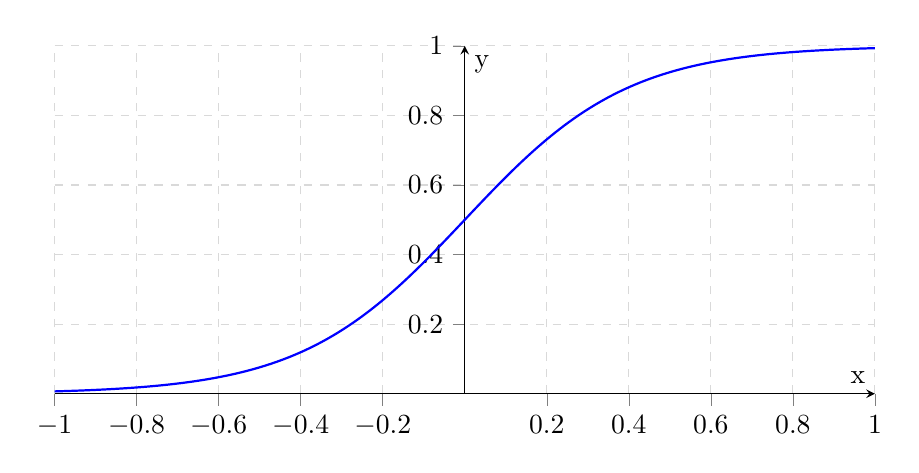
\begin{tikzpicture}
    \begin{axis}[
    	legend pos=north west,
        axis x line=middle,
        axis y line=middle,
        grid = major,
        width=12cm,
        height=6cm,
        grid style={dashed, gray!30},
        xmin=-1,     % start the diagram at this x-coordinate
        xmax= 1,    % end   the diagram at this x-coordinate
        ymin= 0,     % start the diagram at this y-coordinate
        ymax= 1,   % end   the diagram at this y-coordinate
        %axis background/.style={fill=white},
        xlabel=x,
        ylabel=y,
        tick align=outside,
        enlargelimits=false]
      % plot the stirling-formulae
      \addplot[domain=-1:1, blue, thick,samples=500] {1/(1+exp(-5*x))}; 
      %\addlegendentry{$f(x)=\frac{1}{1+e^{-5*x}}$}
    \end{axis} 
\end{tikzpicture}
\end{center}


A seconda del tipo di rete utilizzata cambiano i tipi di neuroni (per esempio quelli LSTM possono essere utilizzati solo con RNN). Quelli utilizzati nel programma sono:\\
\begin{table}[ht]
\centering
\begin{tabular}{| c | c | c |}
\multicolumn {3}{c}{\textbf{Tipi di neurone}}\\
\hline
&\textbf{FFN}&\textbf{RNN}\\\hline
Neurone strato nascosto&Sigmoidea&LSTM\\\hline
Neurone strato di output&Sigmoidea&Sigmoidea\\\hline
\end{tabular}
\end{table}